\section{Time Dilation and Length Contraction}
%By Matt Trawick.

\instructornote{%
By Matt Trawick, 2019.  Time: 60 minutes?

(Activities 1 and 2 are based on a lab I did in Modern Physics for several years.)  

Activity 1 assumes that students have already seen the idea of time dilation and the Lorentz factor $\gamma$, probably by analyzing this exact situation with Anna, Bob, a train, and a flashlight.  This exercise can be their first opportunity to run with this idea a bit on their own, and introduces them to the idea of proper time.

Activity 2 is designed to be a first introduction to the idea of length contraction, showing that it follows directly from time dilation.  It also introduces the idea of proper length.

Activity 3 is an 
}

\makelabheader %(Space for student name, etc., defined in master.tex)

\bigskip

\begin{wrapfigure}[5]{r}{0.35\textwidth}
\begin{center}
\vspace{-0.3in}
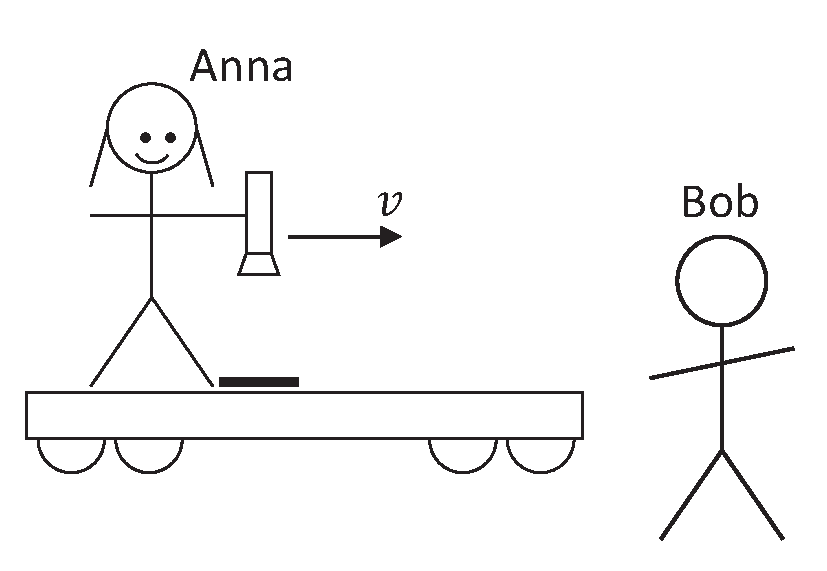
\includegraphics[scale=0.4]{time_dilation_length_contraction/anna_and_bob.eps}
\end{center}
\end{wrapfigure}

\textbf{Activity 1: Time Dilation}

%Consider the case of Anna and Bob that we talked about in class, shown in figures 2.5 and 2.6 on page 10 of Harris.  Suppose that the train is traveling with a speed $v$ such that $\gamma=1.5$.
Anna rides a train towards the east at a speed $v$ such that $\gamma=1.5$.  She turns on a flashlight, which shines onto a mirror directly below it.

\begin{enumerate}[labparts]
\item If Anna measures the light's round trip time to be 6 nanoseconds, what does Bob measure?
\answerspace{0.5in}
\end{enumerate}

\begin{enumerate}[labparts, nosep, resume]
\item Now Anna and Bob try a variation of the experiment.  Anna rides on the train, as before, and the train moves east again, at the same speed $v$, so that $\gamma=1.5$.  But this time Bob holds the flashlight and the mirror.  Both Anna and Bob time the round trip.  What do Anna and Bob each measure for the round trip time $\Delta t$?
\answerspace{0.5in}

\item In an experiment like what Anna and Bob are doing, the shortest measured time between two events (like the emission and detection of a photon) is called the ``proper time.''  What determines who measures the shortest time? Is it who's on the train?  Is it who holds the flashlight?  Is it who holds the mirror?
\answerspace{0.5in}

\item Write a definition of the \textit{proper time,} $\Delta t_0$, between two events.
\answerspace{0.5in}
\end{enumerate}

\begin{wrapfigure}[7]{r}{0.35\textwidth}
\begin{center}
\vspace{-0.4in}
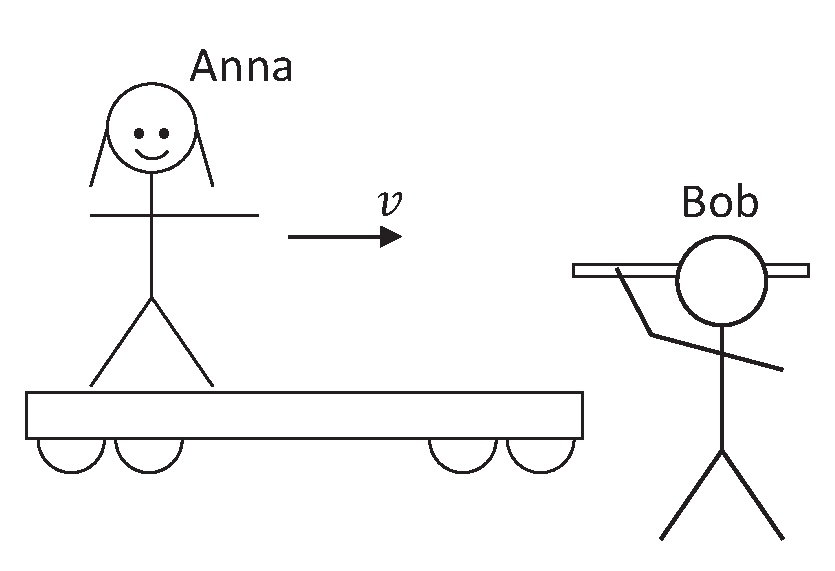
\includegraphics[scale=0.4]{time_dilation_length_contraction/anna_and_bob2.eps}
\end{center}
\end{wrapfigure}

\textbf{Activity 2: What about Length?}

Anna rides the train again at the same speed, and Bob stands on the side, holding a long rod along the direction of the train tracks.  Bob measures the rod to have length $L_0$.  Bob sees Anna traveling past at speed $v$.  Events ``A'' and ``B'' are Anna's nose being even with the left and right ends of the rod, respectively.  Bob measures the time between event A and event B as $\Delta t=L_0 / v$.  

\begin{enumerate}[labparts, nosep]
\item What does Anna say is their relative speed $v$?  (Same as what Bob measures, bigger, or smaller?)
\answerspace{0.4in}
\end{enumerate}

\begin{enumerate}[labparts, nosep,resume]
\item In Anna's frame, what is the time between events A and B, in terms of $\gamma$ and Bob's $\Delta t$?  (Hint: which of the two observers measures the proper time between the two events?  
\answerspace{0.4in}

\item What does Anna infer is the length $L$ of the rod?  (Answer in terms of $L_0$ and $\gamma$.)
\answerspace{0.4in}

\item Bob's measurement, $L_0$, is the ``proper length'' of the rod.  Write a definition of ``proper length'' that highlights why Bob's measurement is different from that made in any other reference frame.
\answerspace{0.5in}
\end{enumerate}

\pagebreak[2]
\textbf{Activity 3: Muon Lifetimes} 

Muons are rare subatomic particles which are not usually found in ordinary matter on Earth.  Muons can be created when protons or atomic nuclei, traveling at high speeds from the sun or other stars, strike the Earth's upper atmosphere and collide with molecules in the air.  As a result of these collisions, there are always muons raining down from the upper atmosphere towards the Earth's surface.

But muons don't last long.  At rest in a laboratory, muons have an average lifetime of only 2.2~$\mu$s, spontaneously decaying into (usually) an electron and two neutrinos.  Given an initial number of muons $N_0$ at time $t=0$, the number of muons $N$ at any later time $t$ is given by
\begin{equation}
N=N_0 e^{-t/\tau},
\end{equation}
where $\tau = 2.2~\mu$s is the muons' average lifetime.  


\begin{enumerate}[labparts]
\item   
Suppose that muons are created in the Earth's atmosphere at a height of 4~km above the surface.  The muons stream towards the ground at a speed of $0.93c$.
In the reference frame of the Earth, how long does it take these muons to reach the ground?
(This is a straightforward question you could have answered in the first week of Physics 131.)
\answerspace{0.8in}

\item What fraction of the original muons should be remaining after this time, according to Equation (1)? 
\answerspace{0.6in}

\item The time $\Delta t$ that you calculated in (a) is the time between two specific events: the muon being created and the muon hitting the Earth's surface.  What reference frame measures the \textit{proper time} $\Delta t_0$ between these two events?  Is it the reference frame of a scientist on Earth, or the reference frame of the muon?
\answerspace{0.4in}

\item What is the time of the journey from the upper atmosphere to the ground in the reference frame of the muon, travelling at speed $0.93c$?
\answerspace{0.8in}

\item What fraction of the original muons should be remaining after this time $\Delta t_0$, in the reference frame of the muons?
\answerspace{0.6in}

\item Whatever causes a muon to decay takes place entirely within the muon itself.  (That's why it's called ``spontaneous'' decay; it's not caused by anything external to the muon.)  
Is the time $t$ that governs the average lifetime of a muon the time as measured in the Earth's reference frame, or the muon's reference frame?  
\answerspace{0.4in}

\item If you measure the fraction of muons that \textit{actually} reach the ground, what fraction will you observe?
(This observation was first done in the 1920s, and was an early experimental confirmation of Einstein's theory of relativity.)
\answerspace{0.4in}

\item One more thing.  In part (d), you probably calculated the muons' $\Delta t_0$ using the idea of time dilation.  Now, try doing it again using the idea of length contraction.  In the reference frame of the muon, what is the distance between the upper atmosphere and the ground?
\answerspace{0.8in}

\item How long does it take the muon to travel that distance?
\answerspace{0.6in}

\end{enumerate}

